\begin{usecase}{Send Welcome Email}
  \ucbasicinfo{Low}{Regular}
  \ucshortdescription{This UC welcomes the user to the platform.}
  \uctrigger{This UC starts when the user account is created.}
  \ucactors{User}{None}
  \ucpreconditions{User account must be created in the system.}
  \ucrelationships{N/A}{N/A}{N/A}
  \ucinputsoutputs{
    \begin{itemize}
      \item \textbf{User name} (Source: System)
      \item \textbf{Welcome email template} (Source: System)
    \end{itemize}
  }{
    \begin{itemize}
      \item \textbf{Welcome email} (Destination: User)
    \end{itemize}
  }
  \ucmainflow{
    \begin{enumerate}
      \item The system fetches the user information.
            \ucinfo{The database is used.}
      \item The system fetches the send welcome email template.
            \ucinfo{The template is filled with the user name.}
      \item The system sends the email with the template.
            \ucinfo{The email is received by the user welcoming them.}
    \end{enumerate}
  }
  \ucexceptions{
    \begin{itemize}
      \item Email server is down.
    \end{itemize}
  }
  \ucconclusion{This UC ends when the user receives an email from us welcoming them.}
  \ucspecialrequirements{An email server must be present to send welcome email.}
\end{usecase}

\begin{figure}[!h]
  \centering
  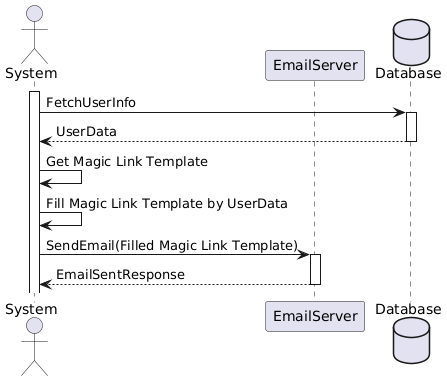
\includegraphics[width=0.5\textwidth]{images/docs/diagrams/sequence-diagrams/all-sequence-diagrams/Send Welcome Email.png}
  \caption{Send Welcome Email Sequence Diagram}
  \label{fig:seq/send-welcome-email}
\end{figure}

The ``Send a Welcome Email Sequence Diagram'', shown in \textbf{Figure~\ref{fig:seq/send-welcome-email}}, shows the process of sending a welcome email to new customers. It begins with the system retrieving user data from the database using the FetchUserInfo function. Once the user data is fetched, the system requests a magic link email template via Get Magic Link Template. The template is then customized with the retrieved user data using Fill Magic Link Template by UserData. The system sends the filled email template to the email server via SendEmail, which delivers the email. Finally, the email server responds with EmailSentResponse, confirming the email's successful dispatch. This sequence ensures personalized and reliable email delivery.
